\documentclass{ctexart}
\usepackage{amsmath}
\begin{document}
\title{计算物理作业 6}
\author{刘畅, PB09203226}
\maketitle

[{\bf 作业 6}]: 对一个实验谱数值曲线 $p(x)$, 自设 $F(x)$, 分别用直接抽样和舍选法
对 $p(x)$ 抽样。比较原曲线和抽样得到的曲线以验证。讨论抽样效率。

\section{算法}
\subsection{直接抽样法}
由于给出的实验谱是一个离散分布, 因此对于直接抽样, 应该用书上离散型随机变量分布的直接抽样法
(1.2.1.1~节). 按照书上讲的, 算法为: 假设对应能量 $\epsilon_i$ 的截面为 $\sigma_i$,
首先将截面 $\sigma_i$ 归一化为几率:
\begin{equation}\label{norm_prob}
p_i = \frac{\sigma_i}{\sum_j\sigma_j}
\end{equation}
这样, 对于 $[0,1]$ 区间中抽到的均匀分布随机数 $\xi$, 如果 $\xi$ 满足
\begin{equation}\label{samp_direct}
\sum_{i=1}^{n-1} p_i < \xi \le \sum_{i=1}^n p_i
\end{equation}
那么抽取的能量值为 $\epsilon_n$.

\subsection{舍选法}
由于这个题要求自选比较函数 $F(x)$, 所以要选择一个容易进行抽样同时又使得抽样效率比较大的.
为此, 选择一个和这个分布的曲线比较接近的矩形函数, 形式为:
\[
F(\epsilon) = \begin{cases}
2713, \quad &2900 \le \epsilon \le 2993 \\
40123, \quad &2994 \le \epsilon \le 3004 \\
443, \quad & 3005 \le \epsilon \le 3010
\end{cases}
\]

要对这个 $F(x)$ 进行直接抽样, 为此需要计算积累函数 $\xi(\epsilon)$
\[
\xi(\epsilon) = \sum_{e = 2900}^{\epsilon} F(e)
\]
由于 $F(\epsilon)$ 是分段常数函数, 因此 $\xi(\epsilon)$ 是分段线性的,
所以非常容易取逆, 记它的逆函数为 $\epsilon(\xi)$.

和上一次作业一样, 舍选法的算法是: 第一步从 $[0,1]$ 区间上抽取均匀分布 $\xi$,
然后按照 $F(\epsilon)$ 分布抽取随机值 $\epsilon$, 第二步判断 $\xi \le
\frac{p(\epsilon)}{F(\epsilon)}$ 是否成立, 若不成立, 返回第一步重新抽样,
否则, $\epsilon$ 就是满足 $p(\epsilon)$ 的一个抽样值.

\section{程序}
由于这个题目的数据在一个文件中, 因此需要首先把文件中的内容读到内存中. 所以
在 \verb|main.c:main()| 中, 首先要做
\begin{verbatim}
    /* read data file into energy[] and count[] */
    i = 0;
    total_count = 0;
    while (fscanf(fin, "%d %d", &energy[i], &count[i]) > 0) {
        total_count += count[i];
        i++;
    }
    nsample = i;
\end{verbatim}
其中, \verb|total_count| 用来记录总的计数, 也就是上面 (\ref{norm_prob}) 中的
$\sum_i \sigma_i$. \verb|energy[]| 是数据文件的第一列, 也就是能量 (eV).
\verb|count[]| 是数据文件的第二列, 也就是计数率 ($\sigma_i$). \verb|nsample|
是实验测得的谱线的总点数.

接下来, 要按照 (\ref{norm_prob}) 中所说的, 归一化截面得到概率. 这是由下面的
代码完成的: (在 \verb|main.c:main()|)
\begin{verbatim}
    /* normalize count rate to get probability */
    for (i = 0; i < nsample; i++) {
        prob[i] = (double) count[i] / (double) total_count;
    }
\end{verbatim}
其中 \verb|prob[]| 对应 (\ref{norm_prob}) 中的 $p_i$.

\subsection{直接抽样法}
按照 (\ref{samp_direct}) 所说, 应该首先得到积累分布
\[
{\rm accum}(n) = \sum^n_{i = 1} p_i
\]
这是由以下代码完成的: (\verb|main.c:main()|)
\begin{verbatim}
    /* compute accumulated probability accum[] */
    accum[0] = prob[0];
    for (i = 1; i < nsample; i++) {
        accum[i] = prob[i] + accum[i-1];
    }
\end{verbatim}
其中, \verb|accum[]| 储存积累分布.

(\ref{samp_direct}) 说, 只要随机生成的 $[0,1]$ 分布 $\xi$ 在 ${\rm accum}(i-1)$
和 ${\rm accum}(i)$ 之间 (可以取到 ${\rm accum}(i)$), 就产生能量的抽样值
${\rm energy}(i)$. 要将这个算法转换成程序, 只要在数组 \verb|accum[]| 中
查找预先生成的随机数 \verb|xi| 就可以了. 为了效率高, 这里采用二分查找法来查找. 代码如下:
(\verb|main.c:sample_direct()|).
\begin{verbatim}
    i = 0;
    j = nsample-1;
    if (xi <= accum[0])
        return energy[0];
    while (i < j-1) {    /* binary search */
        mid = (i + j) / 2;
        if (xi < accum[mid])
            j = mid;
        else if (xi > accum[mid])
            i = mid;
        else
            return energy[mid];
    }
    return energy[j];
\end{verbatim}
这是典型的二分查找算法, 在开始, \verb|i| 和 \verb|j| 设在数组两端.
每次循环, \verb|xi| 都和数组中间的值 \verb|accum[mid]| 比较, 根据
大小关系决定舍去数组的哪一半. 直到 \verb|i| 和 \verb|j| 相遇, 算法停止.

这样直接法的程序就完成了, 为了验证其正确性, 和上一题一样, 由于现有的软件
作出的直方图比较奇怪, 需要自行编写一个例程来实现这个功能. 代码见
\verb|count_freq.c:count_freq()|. 由于这个代码上一次作业已经解释过了,
这里就不重复了.

\subsection{舍选法}
按照前面的算法, 首先要写对 $F(x)$ 进行直接抽样的程序, 为此, 要把 $\xi(\epsilon)$
的反函数求出来, 结果是一个分段线性函数, 这个函数的实现是对 $F(x)$ 直接抽样的函数
\verb|sample_rect| 的最主要部分, 在代码中体现为一组 \verb|if-then-else|
语句 (\verb|main.c:sample_rect()|). (大写的是各种常数.)
\begin{verbatim}
    xi = normfac * rand_norm();
    if (xi <= prob[IDX_MAXPROB_1] * (IDX_ECUTOFF_1+1))
        return xi / prob[IDX_MAXPROB_1];
    else if (xi <= prob[IDX_MAXPROB_1] * (IDX_ECUTOFF_1+1)
         + prob[IDX_MAXPROB_2] * (IDX_ECUTOFF_2-IDX_ECUTOFF_1))
        return (xi - prob[IDX_MAXPROB_1] * (IDX_ECUTOFF_1+1)) /
            prob[IDX_MAXPROB_2] + IDX_ECUTOFF_1 + 1;
    else
        return (xi - prob[IDX_MAXPROB_1] * (IDX_ECUTOFF_1+1) -
            prob[IDX_MAXPROB_2] * (IDX_ECUTOFF_2-IDX_ECUTOFF_1)) /
            prob[IDX_MAXPROB_3] + IDX_ECUTOFF_2 + 1;
\end{verbatim}
其中的 \verb|normfac| 是归一化常数, 由于前面给出的 $F(x)$ 不是归一化的, 因此要除以
$\int_x F(x)$ 才可以看作是概率分布, 这个 \verb|normfac| 就是前面的积分. 由于 $F(x)$
是分段常数函数, 这个积分值非常简单: (\verb|main.c:sample_rect()|)
\begin{verbatim}
    normfac = prob[IDX_MAXPROB_1] * (IDX_ECUTOFF_1+1) +
        prob[IDX_MAXPROB_2] * (IDX_ECUTOFF_2-IDX_ECUTOFF_1) +
        prob[IDX_MAXPROB_3] * (nsample-1-IDX_ECUTOFF_2);
\end{verbatim}

有了这个函数 (\verb|sample_rect()|), 就可以编写舍选法的函数了. 按照前面的算法编码,
其中由于 $F(x)$ 是分段函数, $\frac{p(\epsilon)}{F(\epsilon)}$ 也是分段表示的,
在下面的代码中表现为一组 \verb|if-then-else| 语句. (\verb|main.c:sample_accrej()|)
\begin{verbatim}
    do {
        Nr_total_instance++;
        xi = rand_norm();
        idx = sample_rect(prob, nsample);
        assert(idx >= 0 && idx < nsample);
        if (idx <= IDX_ECUTOFF_1)
            lambda = prob[idx] / prob[IDX_MAXPROB_1];
        else if (idx <= IDX_ECUTOFF_2)
            lambda = prob[idx] / prob[IDX_MAXPROB_2];
        else
            lambda = prob[idx] / prob[IDX_MAXPROB_3];
    } while (xi > lambda);
    Nr_accepted++;

    return energy[idx];
\end{verbatim}
上面的 \verb|Nr_total_instance| 和 \verb|Nr_accepted| 与前一次作业的
功能一样, 用来计量抽样效率.

这样整个程序就完成了.

\section{结果和分析}
下面是直接抽样法的结果:
\begin{center}
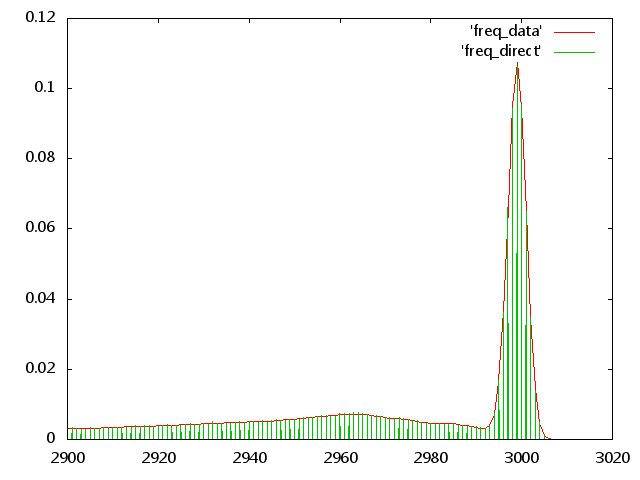
\includegraphics[width=4in]{direct.png}
\end{center}
可以看出, 抽样结果的归一化频率直方图和实验曲线非常一致.

下面是舍选法的结果:
\begin{center}
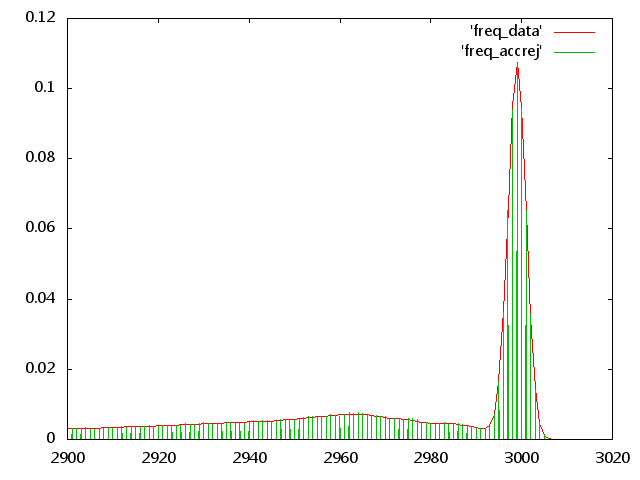
\includegraphics[width=4in]{accrej.png}
\end{center}
同样, 和实验曲线非常一致. 这表示两个方法用在这个问题中都是可行的.

理论上可以证明, 本题舍选法的效率为 $\left(\int_x F(x)\right)^{-1}$, 也就是前面
\verb|normfac| 的倒数, 值为 0.5343352889. 前面程序得出的效率为
\input accrej_efficiency\relax\unskip. 可以看出, 二者非常接近.

\end{document}